\section{Neural Network Architecture}
Network architecture is divided into three components: CNN for character-level
representation, Bi-LSTM and a CRF layer.

\subsection{CNN for Character-level representation}
CNN networks are famous for their appliance in the Computer Vision domain but
they have also demonstrated an ability to extract morphological information
from character of words and encode it into neural
representations\cite{santos2014learning} and \cite{chiu2015named}.
We first create a hash map of all character
that appear in the dataset where the values are arbitrary assigned integer
values. All character from the sentences are then represented using their 
mapped integer values but the padding is also applied on the word level as
shown in Figure \ref{fig:cnn_embed}.
Encoded sentence represents an input which is fed into a trainable character embedding
layer of $C_e \times V$ dimensions, where $C_e$ is the character embedding size,
and $V$ is the number of unique characters in the dataset.

\begin{figure}
  \caption{Character embeddings layer followed by a 1-D convolutional layer.
  Max pool layer with stride=2 and size=2 is applied after the convolution.}
  \label{fig:cnn_embed}
  \centering
    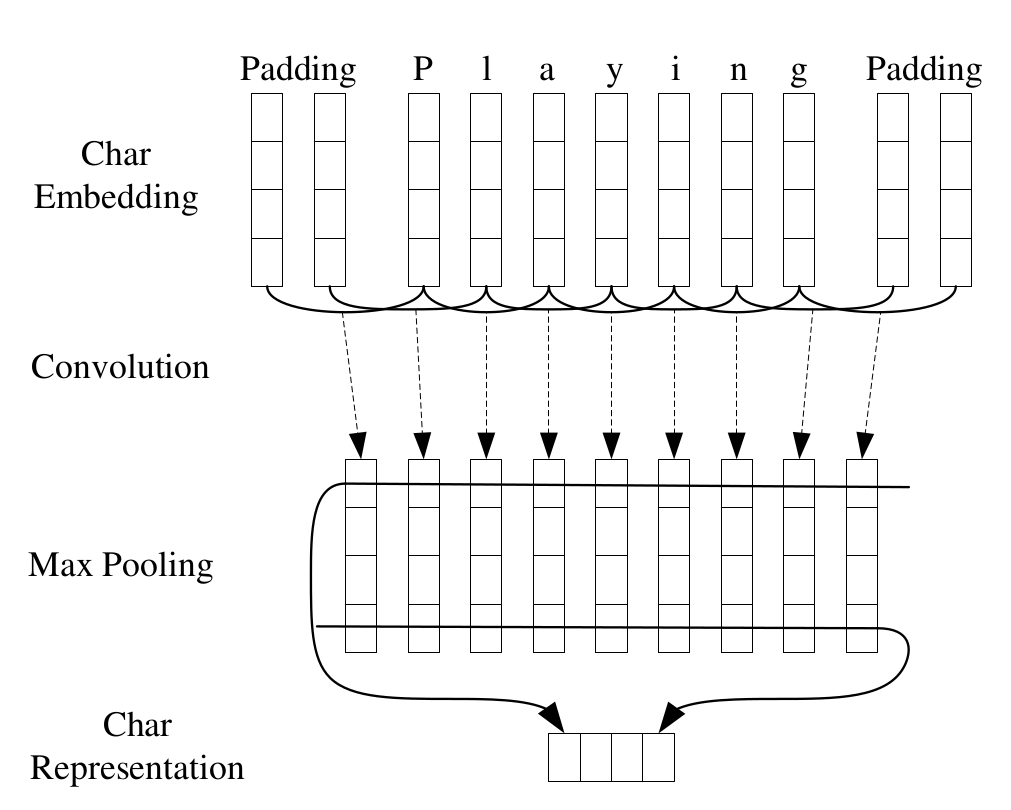
\includegraphics[width=0.5\textwidth]{cnn_embed.png}
\end{figure}

Before the vectors are passed to a CNN layer, the
dropout\cite{srivastava2014dropout} layer is
applied. Dropout is a technique that is used for preventing the model from
overfitting. One dimensional convolution is applied after the dropout which
yields character feature vectors. Generated vectors are concatenated with the word
embedding vectors. Word embeddings are pre-trained vectors
that model the inter word relatedness. Some of the most frequently used are
\textit{word2vec}\cite{mikolov2013distributed}, \textit{Glove}
variants\cite{pennington2014glove} and
Senna\cite{collobert2011natural}. Authors have also experimented with randomly sampled word
embeddings and the results were poor in comparison with the pre-trained vectors
so I have only focused on the former.

\subsection{Bi-directional LSTM}

\subsubsection{LSTM}
The main idea behind RNNs lies in retaining the information from "history".
In the context of NLP, history refers to observing the whole context of the
sentence and not just one part of it. Despite the promising results in short
sentences, RNN losses its performance dramatically with the increasing sentence
length due to the gradient vanishing\cite{bengio1994learning}
and exploding problems \cite{pascanu2013difficulty}.

\begin{figure}
  \caption{LSTM cell architecture}
  \label{fig:lstm}
  \centering
    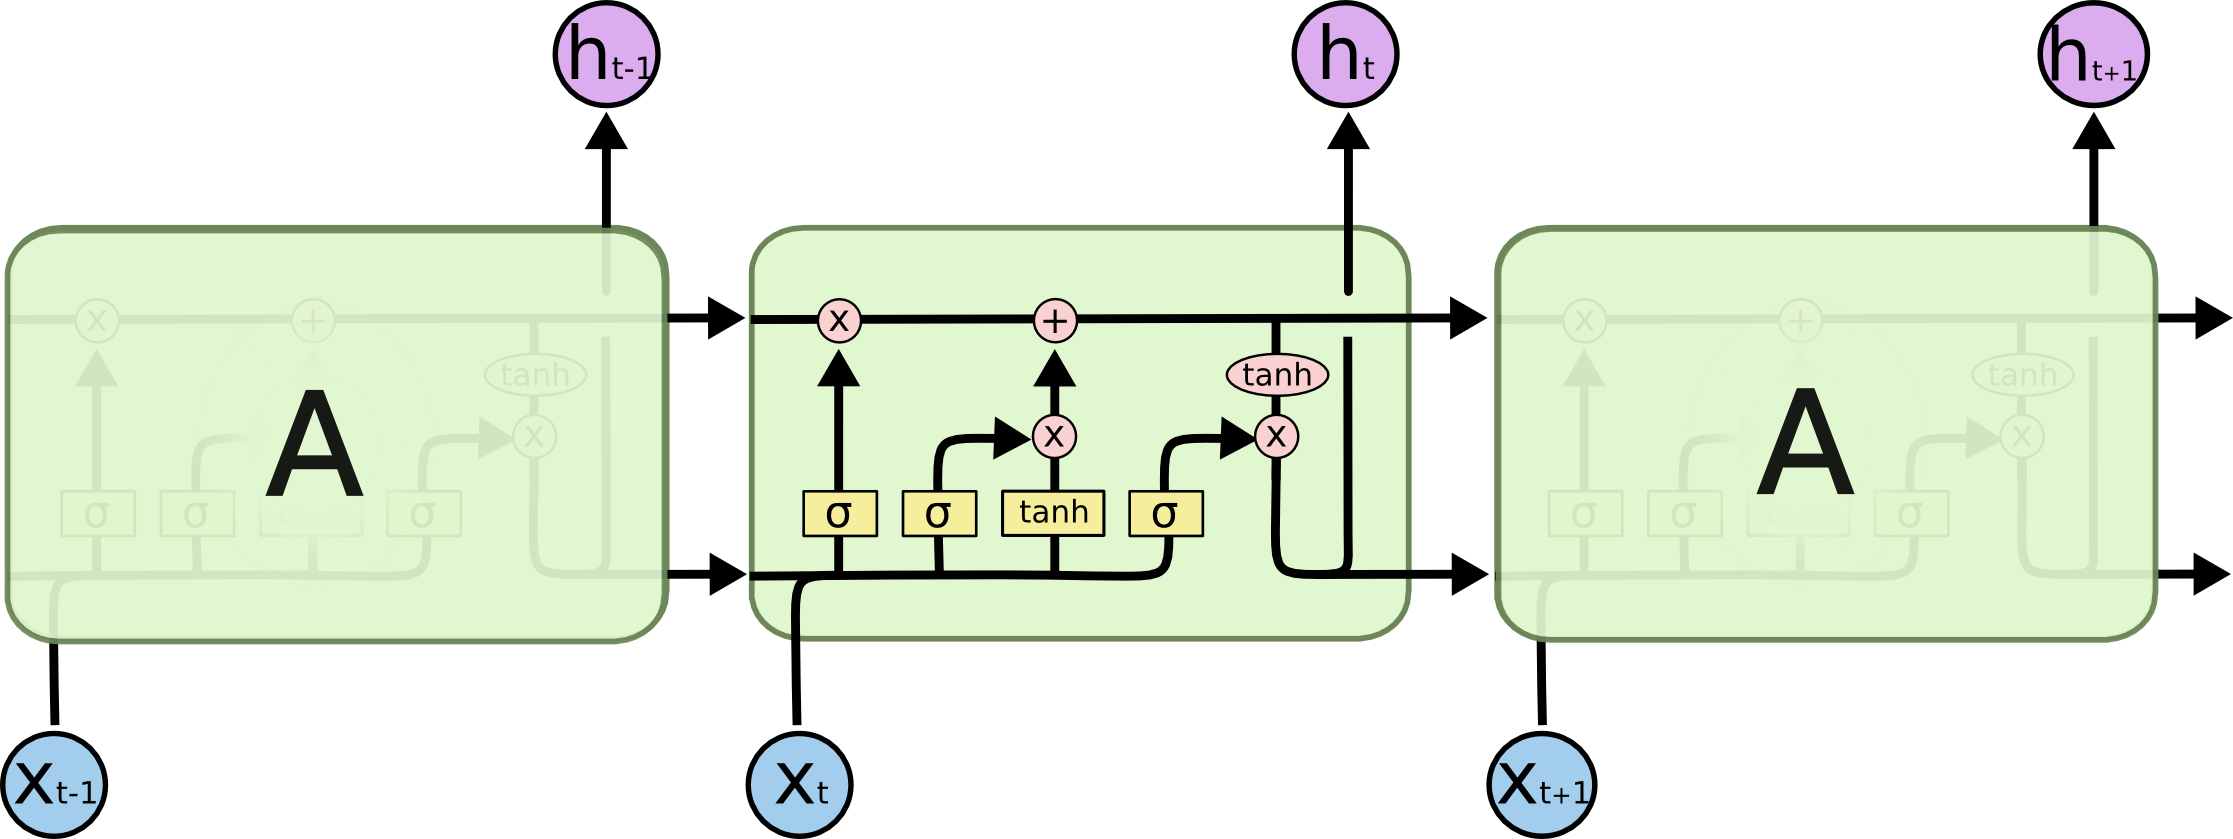
\includegraphics[width=0.6\textwidth]{lstm.png}
\end{figure}

LSTMs were designed with the purpose of correcting the RNNs shortcomings. The LSTM
cell unit is composed of four gates which control the proportion of
information to forget and to pass on to the next time step. In Figure
\ref{fig:lstm} we can see the LSTM cell structure. The first fork from the left
is a forget gate which regulates the old information retention. Next two forks 
describe how new and the accumulated information from the past are joined
together. The final fork can be seen as a mix of the filtered input with the
updated cell state which will be the final cell output. Equation that model the
LSTM cell at the time step $t$ are the following:

\begin{align*}
        i_t &= \sigma\left(W_ih_{t-1} + U_{i}x_t + b_i\right)\\
        f_t &= \sigma\left(W_fh_{t-1} + U_{f}x_t + b_f\right)\\
        \hat{c_t} &= tanh\left(W_ch_{t-1} + U_{c}x_t + b_c\right)\\
        c_t &=  f_t \odot c_{t-1} + i_t \odot \hat{c_t}\\
        o_t &= \sigma\left(W_oh_{t-1} + U_{o}x_t + b_o\right)\\
        h_t &= o_t \odot tanh(c_t)
\end{align*}

$\sigma$ is a sigmoid function and $\odot$ represents an element-wise
multiplication. $x_t$ is a vector of an arbitrary dimension and $h_t$ is the
accumulated cell information up to a time step $t$. $U_i$, $U_f$, $U_c$, $U_o$
denote the weight matrices of different gates for input $x_t$, and
$W_i$, $W_f$, $W_c$, $W_o$ are the weight matrices for hidden state $h_t$.
$b$ terms are the corresponding bias vectors.

\subsubsection{Bi-LSTM}
Although LSTM can successfully capture the past context, it is sometimes good
to have an insight at the future sentence context. Bi-LSTMs model
this by adding a an extra LSTM layer which has a reversed information flow
meaning that the information is propagated from the end of the sentence towards
the beginning. Output of a Bi-LSTM is a concatenated vector of the two opposite
LSTM layers.

\subsection{Conditional Random Fields}
Sequence labelling tasks have correlations between labels in neighbourhoods so
it is a good approach to jointly decode the best chain of labels for a given
sequence. CRFs enable us to model label sequences jointly instead of coding
each label independently. Joint probability is modeled according the following
equation:
\begin{align*}
    p(y | x, w) &= \frac{1}{Z(x, w)} \prod_c \phi(y_c | x, w)\\
    \phi(y_c | x, w) &= \exp(w_c^T \theta(x, y_c))
\end{align*}
where $\theta(x, y_c)$ is a feature vector derived from the global inputs $x$
and the local set of labels $y_c$.

CRF is trained using a maximum conditional likelihood estimation. For a
training set $\{(x_i, y_i)\}$, the logarithm of the likelihood is given by:
\begin{align*}
    L(w) = \sum_i \log p(y | x; w)
\end{align*}

Training procedure chooses parameters such that the log-likelihood is
maximized.

Decoding is defined as a search for the label sequence $y^*$ with the highest
conditional probability:
\begin{align*}
    y^* &= \arg\max\limits_{y \in \gamma(x)} p(y | x; w)
\end{align*}
where $\gamma(x)$ denotes the set of possible label sequences for $x$.
The main network architecture can be seen in Figure \ref{fig:pipeline}.

\begin{figure}
  \caption{The main network architecture. Dashed layers indicate dropout layers
  applied both on the input and output vectors of Bi-LSTM. Word and character
  embeddings are concatenated before inputed in the Bi-LSTM}
  \label{fig:pipeline}
  \centering
    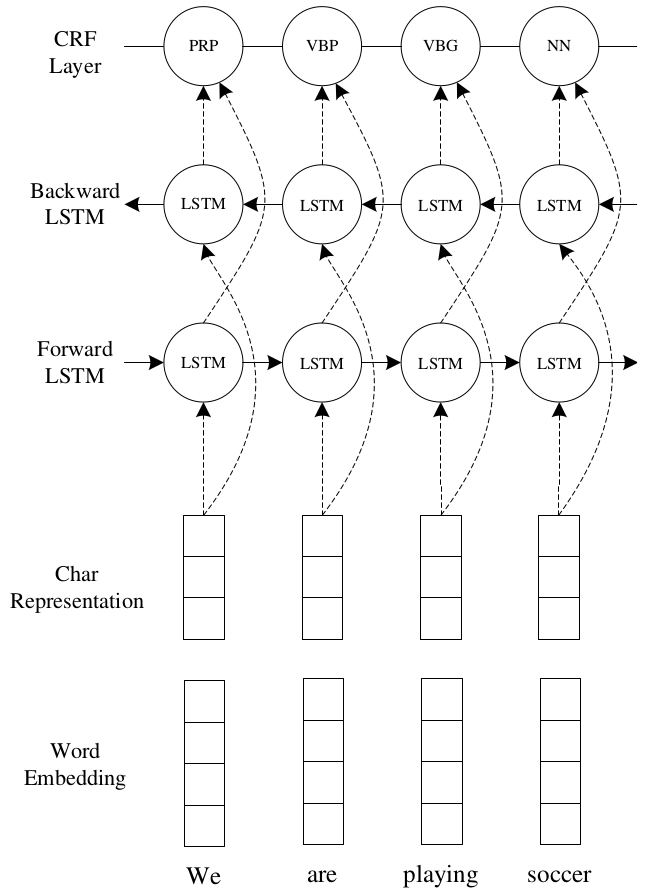
\includegraphics[width=0.6\textwidth]{pipeline.png}
\end{figure}

